\documentclass[tikz]{standalone}
\usetikzlibrary{automata,positioning}
\begin{document}
  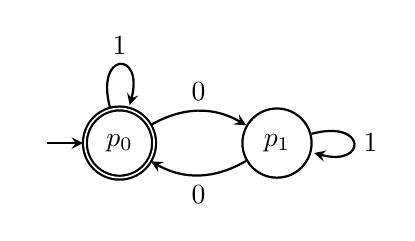
\begin{tikzpicture}[>=stealth,node distance=2cm,on grid,auto, thick, initial text=]
    \node[state,initial,accepting] (p_0) {$p_0$};
    \node[state] (p_1) [right=of p_0] {$p_1$};
    
    \path[->]
    (p_0) edge [loop above] node {1} (p_0)
    (p_0) edge [bend left] node {0} (p_1)
    (p_1) edge [loop right] node {1} (p_1)
    (p_1) edge [bend left] node {0} (p_0);
  \end{tikzpicture}

\end{document}